\section{PSR J1513$-$5908: Characterizing a Soft $\gamma$-ray Pulsar with Single-Altitude Model}
\paperref{
This section is based on work done for
``Broad-Band KeV to MeV Characteristics of Soft $\gamma$-Ray Pulsar PSR J1513$-$5908''
\citep{hartogJ1513}.}

\begin{figure}[htbp]
\begin{center}
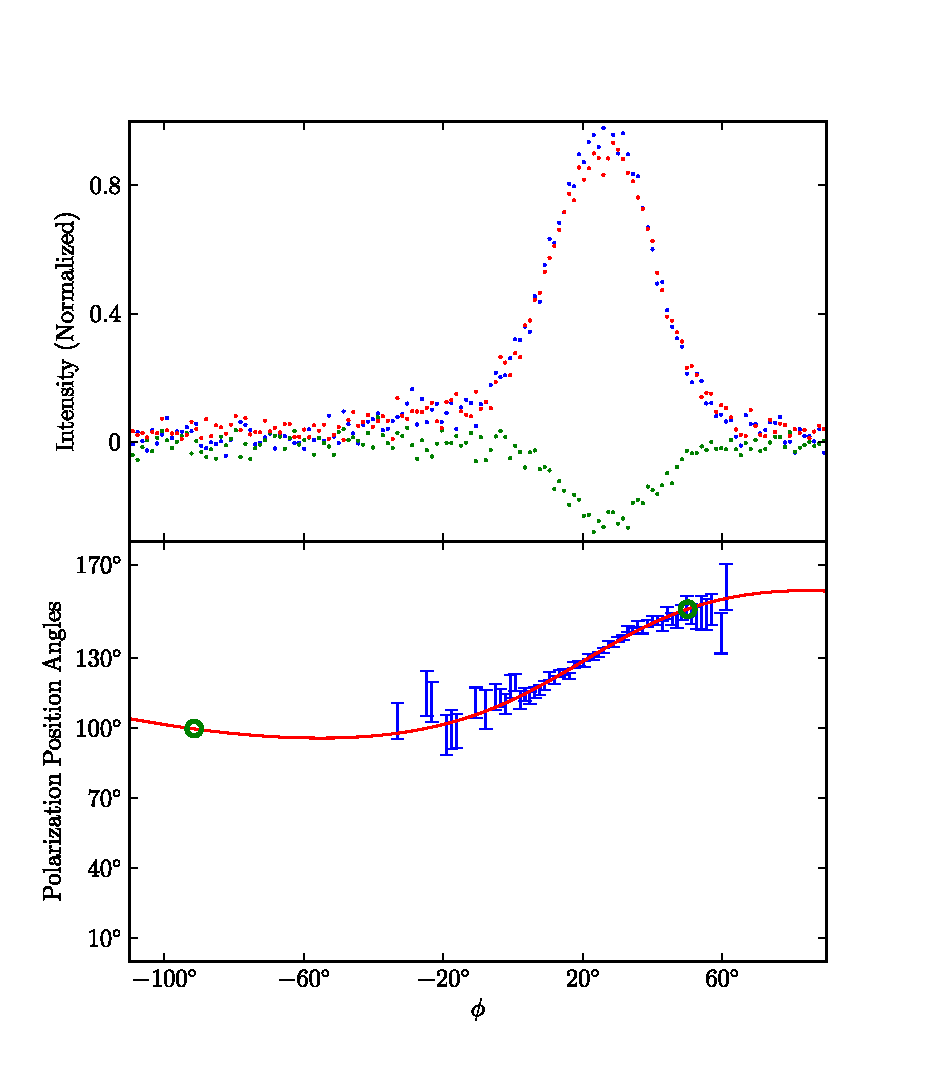
\includegraphics[scale=.8]{chapters/multiWaveLength/figures/intAndPAJ1513alpha153zeta133.eps}
\caption[Intensity and polarization data for PSR J1513$-$5908 overlaid with model]{\label{fig:intAndPAJ1513alpha153zeta133}
Figure taken from \cite{hartogJ1513}.
Intensity and polarization data for PSR J1513$-$5908 overlaid with model.
In the upper panel, blue points are total intensity data, red points are linear polarization intensity data,
and green points are circular polarization intensity data for PSR J1513$-$5908 at 20 cm.
In the bottom panel, blue error bars are polarization position angles
used in the fit. 
The red solid line is the fit model
polarization with $R=0.24R_{\rm{LC}}$, $\alpha=153^{\circ}$, and $\zeta=133^{\circ}$. 
Empty circles mark phase of emission from open field lines.
}
\end{center}
\vskip -0.2truecm
\end{figure}

\begin{figure}[t!!]
\begin{center}
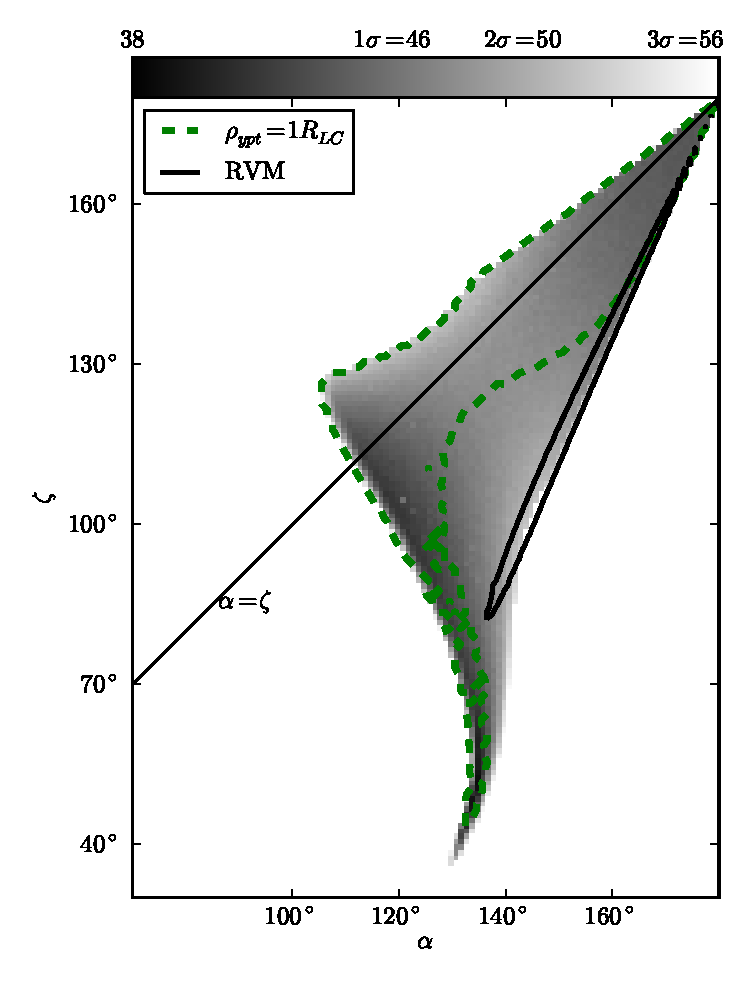
\includegraphics[scale=.8]{chapters/multiWaveLength/figures/J1513-5908Map.eps}
\caption[Map of $\chi^{2}$ for PSR J1513-5908 fit to radio polarization in the $\alpha$-$\zeta$ plane]{\label{fig:J1513-5908Map}Figure taken from \cite{hartogJ1513}.
Map of $\chi^{2}$ for PSR J1513-5908 fit to radio polarization in the $\alpha$-$\zeta$ plane.
Overlaid are  $3\sigma$ above $\chi^2_{\rm min}$ contour for
zero altitude RVM fit (black) and $3\sigma$ above $\chi^2_{\rm min}$ contour for the assumption that emission must come from the formal open
zone.
}
\end{center}
\vskip -0.2truecm
\end{figure}

\begin{figure}[htbp]
\begin{center}
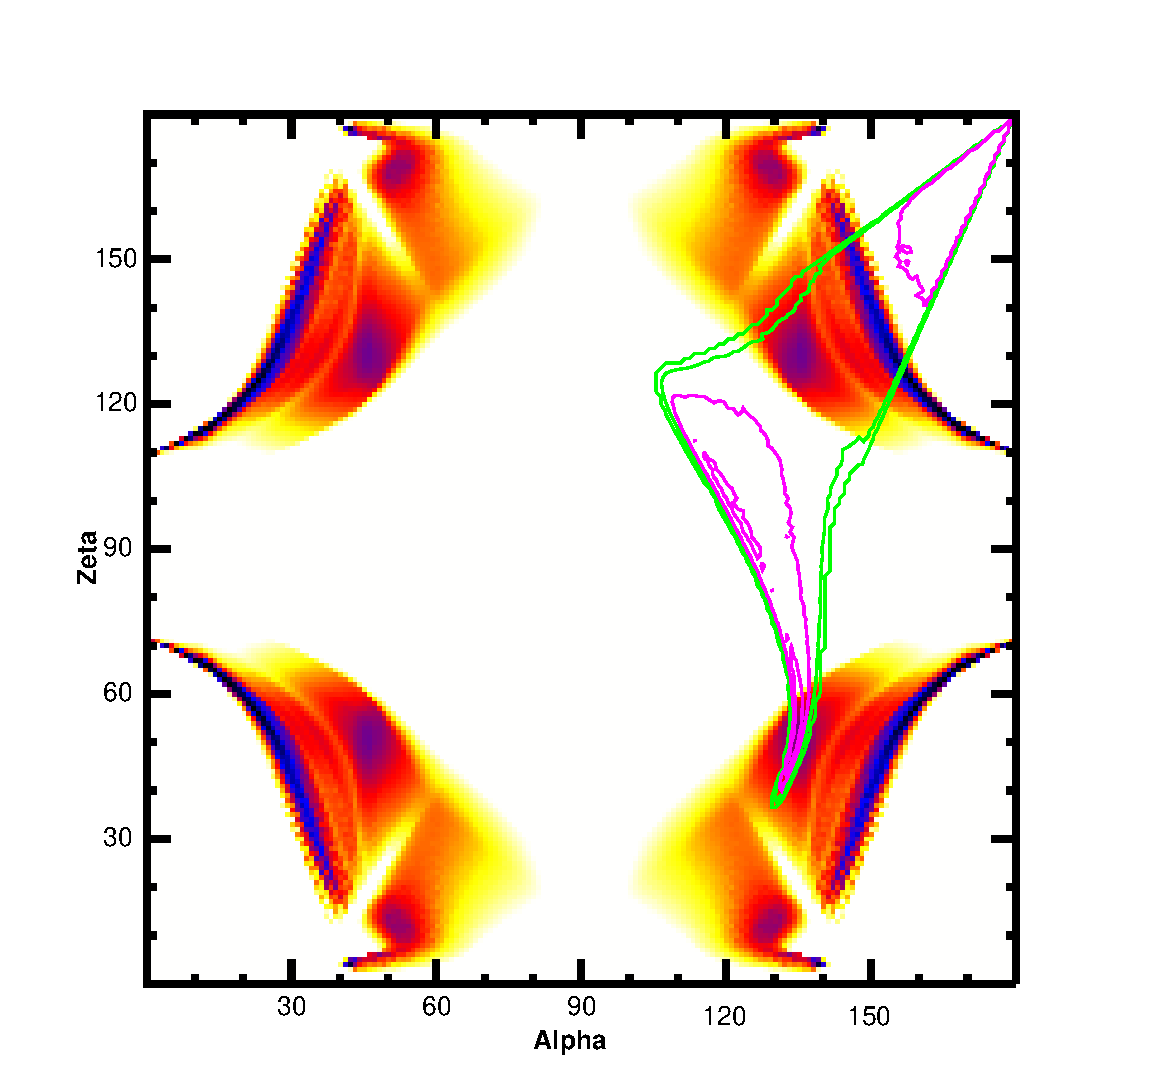
\includegraphics[scale=.8]{chapters/multiWaveLength/figures/BJ1513_w10.eps}
\caption[Pulsar geometry and emission modeling fit map of an outer gap model and radio polarization model 
for PSR J1513$-$5908 in
the $\alpha$--$\zeta$ plane of the pulsar]{\label{fig:BJ1513_w10}
Figure taken from \cite{hartogJ1513}.
Pulsar geometry and emission modeling fit map of an outer gap model 
and radio polarization model for PSR J1513$-$5908 in
the $\alpha$--$\zeta$ plane. Contours show the polarization
fit of the $0.5\sigma$ and $1.0\sigma$ regions in magenta;
and the $2.0\sigma$ and $3.0\sigma$ regions in green.
A wide range of geometries is allowed by these polarization data,
including the best $\gamma$-ray fits. Good fits must also match the
phase of the magnetic dipole axis (see text).
}
\end{center}
\vskip -0.2truecm
\end{figure}

\begin{figure}[htbp]
\begin{center}
\includegraphics[width=\textwidth]{chapters/multiWaveLength/figures/J1513_lc.eps}
\caption[Radio and $\gamma$-ray light curves of PSR J1513$-$5908 with model light curve for $\alpha=153^\circ$, $\zeta=133^\circ$]{\label{fig:J1513_lc}
Figure taken from \cite{hartogJ1513}.
Radio and $\gamma$-ray light curves of PSR J1513$-$5908 with model light curve for $\alpha=153^\circ$, $\zeta=133^\circ$.
A single
peak dominates since the line of sight skims the $\gamma$-ray caustic. The
radio emission altitude is 0.24$R_{\rm LC}$ and polarization and
$\gamma$-ray fits both indicate that the magnetic axis (green upwards arrow)
leads the radio peak by $\phi=0.08$.
}
\end{center}
\vskip -0.2truecm
\end{figure}



The paper ``Broad-Band KeV to MeV Characteristics of Soft $\gamma$-Ray Pulsar PSR J1513$-$5908''
\citep{hartogJ1513} aims to do a 
spectral study covering 2 KeV to 1 GeV including 
updated {\it Fermi} data and revisited archival RXTE-PCA and HEXTE data
along with historic CGRO-COMPTEL data of the pulsar PSR J1513$-$5908 (PSR B1509$-$58).
The pulsar was also analyzed using radio polarization data.

The polarization data analyzed is 1.4 GHz data.
The pulsar PSR J1513$-$5908 has a period of 151 ms.
Also noted in the paper is
an extra component in the radio intensity of PSR J1513$-$5908
before the peak of the main pulse.
We had hoped to model this component using polarization
but the scatter of the data was too large to derive
useful fit results.

The typical retarded dipole with photons projected tangent to the magnetic
field lines is used to calculate the position 
angles of the polarization.  Further, models used here
extrapolate from the classical RVM allowing emission from finite
radial altitudes above the surface of the neutron star with relativistic and sweep-back effects.  
Allowed altitudes ranged between
$.002R_{\rm{LC}}$ (the radius of the neutron star assuming $R_{\rm{NS}}\sim 15$ km) to $.9R_{\rm{LC}}$.

Figure~\ref{fig:intAndPAJ1513alpha153zeta133} shows the polarization position angle sweep and intensity
profile for 20 cm data.  The sweep is relatively simple and shows no signs of orthogonal
mode jumps or multiple altitude.  RVM fits relatively well to the polarization with
$\chi^2_{\rm{min}}=44$ for Degree of Freedom=DOF$=55-4$.  The four fit parameters are $\alpha$, the angle between
the magnetic axis and rotation axis, $\zeta$, the viewing angle as measured from the rotation
axis and the horizontal and the vertical offsets in the 
polarization angles.  The best fit model
with finite altitude has $\chi^2_{\rm{min}}=39$ for DOF$=55-5$ although the best fit model might
not be the most physically viable model as will be discussed later.  The solid red line in
Figure~\ref{fig:intAndPAJ1513alpha153zeta133} is a finite-altitude model at $\alpha=153^\circ$,
$\zeta=133^\circ$, and $R=0.24R_{\rm{LC}}$ with $\chi^2=48$.  Green circles on the
solid red line mark the expected end of emission based on a formal open zone assumption.


Figure~\ref{fig:J1513-5908Map} shows the best fit $\chi^2$ surface map projection in the
$\alpha$-$\zeta$ plane for the single-altitude model.  
The $3\sigma$ contours for the RVM fit are
overlaid on the color map in black.  Additionally, on this panel is a green contour that
encloses the model parameters for which model emission phase is equal to or greater than
the emission phase seen in the data.  The model emission phase is defined by the emission
from the classic open field lines.  Overlap between these contours is minimal.  This indicates
a physical need to increase emission phase from RVM either by increasing the altitude of emission
or widen the open zone cap.

Following \cite{romani2010constraining} we fit the $\gamma$-ray
light curve using the $\chi_3$ statistic. While PSR J1513$-$5958 is
very energetic, implying a small gap and emission close to the last closed
field lines, we find appreciably better light curves for a modest gap width,
$w=0.05-0.1$. In Figure~\ref{fig:BJ1513_w10}, the background color scale shows the goodness of
fit for an outer gap  model with $w=0.1$. Overlaid are
contours from the radio fitting. To be a viable model, the $\gamma$-ray fit
must lie inside the radio contours. Since the polarization presents a simple sweep, this
is not very constraining, with a wide range of geometries compatible at the
$3\sigma$ level. However, the polarization fit also tightly constrains
the phase of the magnetic axis relative to the radio intensity peak. For
a viable model, this should match as well.

The strip of best $\gamma$-ray fits crosses the radio-allowed region
along $\alpha=153^\circ$ and $\zeta=145^\circ$ to 
$\alpha=156^\circ$ and $\zeta=128^\circ$
with $\chi_3<4.5$. In
this region the phase of the magnetic axis ranges from $-0.06$ to $-0.08$
(in fractions of a period)
and the radio emission altitude varies from $0.1$ to $0.3R_{\rm LC}$.
In Figure~\ref{fig:J1513_lc}, we show the fit $\gamma$-ray light curve 
for $\alpha=153^\circ$ and $\zeta=133^\circ$.
The radio fit altitude is $0.24R_{\rm LC}$ and the polarization
fit is $1.2\sigma$ from its minimum. In this region {\it both}
the $\gamma$-ray and polarization fits place the magnetic dipole axis
0.08 before the radio peak.  A second region of plausible $\gamma$-ray fits
(with $\chi_3 \approx 5.4$) lies close to the polarization fit minimum.
In this region, $\alpha=135^\circ$ and $\zeta=51^\circ$ 
and the $\gamma$-ray light curve, while
dominated by a single peak, has a tail to phase $0.5$.  However the fit magnetic
axis phases do not agree (-0.03 for $\gamma$-ray, 0 for radio) and the radio
altitude is quite high, 0.75 to 0.85$R_{\rm LC}$. At this altitude the details
of the magnetic structure are less reliable; so we prefer the lower altitude
solution with the correct phase match. At this lower altitude, there is
also room for the field lines to open within the light cylinder, giving
a y-point radius $<1$ and a larger effective $w$.

